% mapgis2shp paper -- manuscript for Earth Science Informatics (Software article).
% Standard article class; compiles on any TeX installation without custom .cls.
% Compile:  pdflatex paper && pdflatex paper   (bibliography is inline)
\documentclass[11pt,a4paper]{article}

\usepackage[margin=2.5cm]{geometry}
\usepackage{graphicx}
\usepackage{booktabs}
\usepackage{amsmath}
\usepackage{url}
\usepackage{xcolor}
\usepackage{hyperref}
\hypersetup{colorlinks=true,linkcolor=blue,citecolor=blue,urlcolor=blue}

\title{mapgis2shp: an open-source Python toolkit for MapGIS 6.x/67 binary vector formats with native-export validation}

\author{%
  Shijie Li\thanks{Co-corresponding author. Email: \texttt{1045105061@qq.com}}, %
  Haiyang He\thanks{Co-corresponding author. Email: \texttt{hehaiyangcugb@foxmail.com}}, %
  Xu Sun, Haoyang Qin, Xiaoyu Liu, Yilin Feng, Zengyun Zuo \\[2pt]
  \small Xi'an Mineral Resources Survey, China Geological Survey, Xi'an, China%
}
\date{}

\begin{document}
\maketitle

\begin{abstract}
\noindent
MapGIS is widely used in Chinese geological surveying, but its legacy binary vector formats---\texttt{.wt} (point), \texttt{.wl} (line), and \texttt{.wp} (polygon)---lack native support in mainstream open-source geospatial tools. We present \textbf{mapgis2shp} (PyPI distribution \texttt{mapgis2shp}, import name \texttt{pymapgis}), an Apache-2.0 Python toolkit for these formats. Version 2.4.0 supports bidirectional conversion between MapGIS binaries and GeoPandas-supported formats. It also provides coordinate-reference-system (CRS) inference, polygon-topology reconstruction, optional graphic-parameter decoding, and structural parsers for the MapGIS symbol and line-style libraries. We evaluate the reader path against official MapGIS 6.7 exports on two datasets. Across 36 real survey layers comprising 16{,}874 features, feature counts and attribute schemas match exactly, all aligned geometries meet the type-specific coincidence criteria, and the unweighted mean of layer-level attribute-equivalence rates is 99.9995\%; only two of 95{,}006 compared cells are classified as residual mismatches, both consistent with coarse rounding of very small floating-point values in the native export. On the benchmark machine, sequential reading of this corpus took a median of 0.848~s and reached 129.5~MiB peak working set (22.2~MiB above the post-import baseline). On a 400~MB polygon file of 78{,}873 features, the reader attains 99.73\% coverage intersection-over-union and produces zero invalid geometries versus three in the post-processed reference export. This large-file test also bounds the main reconstruction artefact: heuristic arc merging increases summed polygon area by 1.66\% through overlaps, whereas the union-level coverage difference is 0.27\%. The examined native exports additionally discard floating-point precision, string padding, and CRS metadata retained by the reader. Writer and graphic-library functionality are covered by regression tests, with Reader--Writer--Reader round-trip checks for the write path; these checks are separate from native-export validation. mapgis2shp thus provides an open route to access, convert, and archive legacy MapGIS data while making its geometric and validation boundaries explicit.

\medskip
\noindent\textbf{Keywords:} MapGIS; reverse engineering; vector format; GeoPandas; shapefile; geological survey; open source
\end{abstract}

\section{Introduction}

\subsection{Motivation}
MapGIS (Zondy Cyber, Wuhan) is the de facto geographic information system of the Chinese geological-survey community, underpinning regional geological mapping, mineral exploration, and engineering geology~\cite{ma2012,han2012}. Its native vector storage---the 6.x/67 generation's \texttt{.wt} (point), \texttt{.wl} (line), and \texttt{.wp} (polygon) binary files---is closed: the vendor does not publish the on-disk layout, and the format is distinct from the later MapGIS K9/10 ``open data format''. Consequently, survey data held in these files cannot be read by the open-source geospatial stack (GDAL/OGR, GeoPandas, QGIS, GRASS) without the proprietary software. This lock-in impedes reproducible analysis, data sharing, and long-term archival---issues that have been repeatedly raised for proprietary geoscience formats in the open-science literature.

\subsection{The interoperability gap}
Our search of the official GDAL/OGR vector-driver index found no MapGIS driver for the legacy binary formats, and searches of the \texttt{OSGeo/gdal} issue tracker and pull requests found no references to ``MapGIS'' or ``ZondyCyber''~\cite{gdalwebsite}. Because QGIS, GRASS, SAGA, and WhiteboxTools rely on GDAL/OGR for vector I/O~\cite{warmerdam2008}, this absence prevents them from opening \texttt{.wt}/\texttt{.wl}/\texttt{.wp} files natively through their usual vector-I/O path. The vendor instead documents an ASCII ``plain-code'' exchange format and the newer MapGIS~10 open format; neither directly supplies an open-source reader for the legacy binary layout considered here.

\subsection{Related work}
\label{sec:related}
Several open-source MapGIS readers predate this work and warrant explicit acknowledgement. The present software, mapgis2shp, is the matured and validated successor to the first author's earlier single-file reader \texttt{pymapgis}~\cite{pymapgis2022}, which first published a byte-level format description. The validated reader added coordinate-reference inference, a vectorised parser, polygon-topology reconstruction, and independent validation against the reference implementation; the current 2.4.0 release further adds native-format writing, expanded graphic-parameter decoding, and graphic-library parsers. \texttt{MathsionYang/MapGIS2ArcGIS}~\cite{mathsionyang2019} (2019, C\#) independently parses the \texttt{.wl} structure at the record level. \texttt{BenChao1998/ConvertMapGIS}~\cite{convertmapgis2025} (2025) is an independent third-party derivative of \texttt{pymapgis}---not authored by the present authors---that republishes a detailed byte-level specification in its README and adds a graphical converter. \texttt{WenboWong/OGC.net}~\cite{ogcnet2021} (2021, C\#) and earlier C\# format-bridge tools are further examples. Chinese-language academic literature has also analysed the format programmatically---notably Wang~\cite{wang2013} on reading the \texttt{.wt} point file, Wu and Feng~\cite{wufeng2006} on MapGIS--Geodatabase conversion, and Chen~\cite{chen2000} on MapGIS format conversion in MATLAB---but these are short application notes: none ships an open-source reader, none publishes a byte-level specification, and none validates output correctness.

Methodologically, this work belongs to a well-established genre of open-source readers for closed or under-documented scientific binary formats, including \texttt{sas7bdat} for SAS files~\cite{shotwell2011}, \texttt{python-ags4} for AGS4 geotechnical files~\cite{senanayake2022}, and the long-running GDAL library~\cite{warmerdam2008} for numerous proprietary GIS formats. GeoSciML provides a comparable geoscience-format specification effort~\cite{sen2005}, and van~den~Bos~\cite{vandenbos2014} discusses binary-format reverse-engineering methodology in general terms. Within the target journal, format-bridge software such as ArcGMT~\cite{wright1998} establishes precedent for this type of contribution.

Across the tools and publications examined, we found no public report combining independent validation against the reference implementation, coordinate-reference inference, and a reproducible validation harness. The present work addresses this joint gap; it does not claim priority for byte-level parsing or shapefile conversion alone.

\subsection{Contributions}
This paper makes the following contributions:
\begin{enumerate}
  \item A maintained Apache-2.0 implementation of MapGIS 6.x/67 interoperability. The validated core reads \texttt{.wt}, \texttt{.wl}, and \texttt{.wp} files into standard \texttt{geopandas.GeoDataFrame} objects; version 2.4.0 additionally writes native binaries and exposes graphic parameters and graphic-library structures.
  \item A coordinate-reference-inference and polygon-topology-reconstruction pipeline that restores information needed for open-source spatial analysis but omitted by the examined native exports.
  \item A two-tier native-export validation of the reader path: 36 small and medium layers (16{,}874 features; geometric coincidence within the stated tolerance; 99.9995\% mean per-layer attribute equivalence with two residual mismatches) and one 400~MB polygon file (78{,}873 features; 99.73\% coverage IoU).
  \item An explicit reproducibility and regression record: a 36-file reader baseline, Reader--Writer--Reader round-trip checks, unit and integration tests, the historical native-validation scripts and reports preserved in the repository record, and a reproducible reader-performance benchmark with raw timing and memory outputs.
\end{enumerate}
The contribution is the integrated implementation and its evidence base, not a claim of priority for byte-level parsing or shapefile conversion alone.

\section{Background: the MapGIS 6.x/67 binary formats}
All three file types share a common top-level organisation: an 8-byte magic header (\texttt{WMAP`D22} for points, \texttt{WMAP`D21} for lines, and \texttt{WMAP`D23} for polygons), a 4-byte file-identifier int32, and a 4-byte \texttt{data\_start} offset that locates a 10-entry index table. Each index entry occupies 10~bytes, of which the first 8 hold a \texttt{(start, volume)} pair describing one sub-data region. Numeric values are little-endian, and strings are GBK-encoded.

The point section stores 93-byte records, with X and Y as little-endian doubles at offsets 7--14 and 15--22 respectively. The line and polygon files share a 57-byte arc-index record (point count at offset 10--13; byte offset into the coordinate section at 14--17) followed by a coordinate section of 16-byte XY pairs. The polygon file additionally stores a 24-byte topology record whose bytes 8--15 carry the left and right polygon identifiers of each arc, from which closed rings, shells, and holes are reconstructed.

CRS information resides at fixed offsets in the file header: projection type at byte~109, ellipsoid at byte~110, scale denominator (double) at byte~143, and---for projected CRSes---the central meridian and standard parallels, encoded as \texttt{DDDMMSS.sss} doubles, from byte~151 onward. The byte-level reference accompanying the software documents these core sections and the currently supported graphic-parameter layouts. Figure~\ref{fig:layout} summarises the geometry, topology, and attribute layout; it is not an exhaustive map of every graphic-parameter or graphic-library structure.

\begin{figure}[h]
\centering
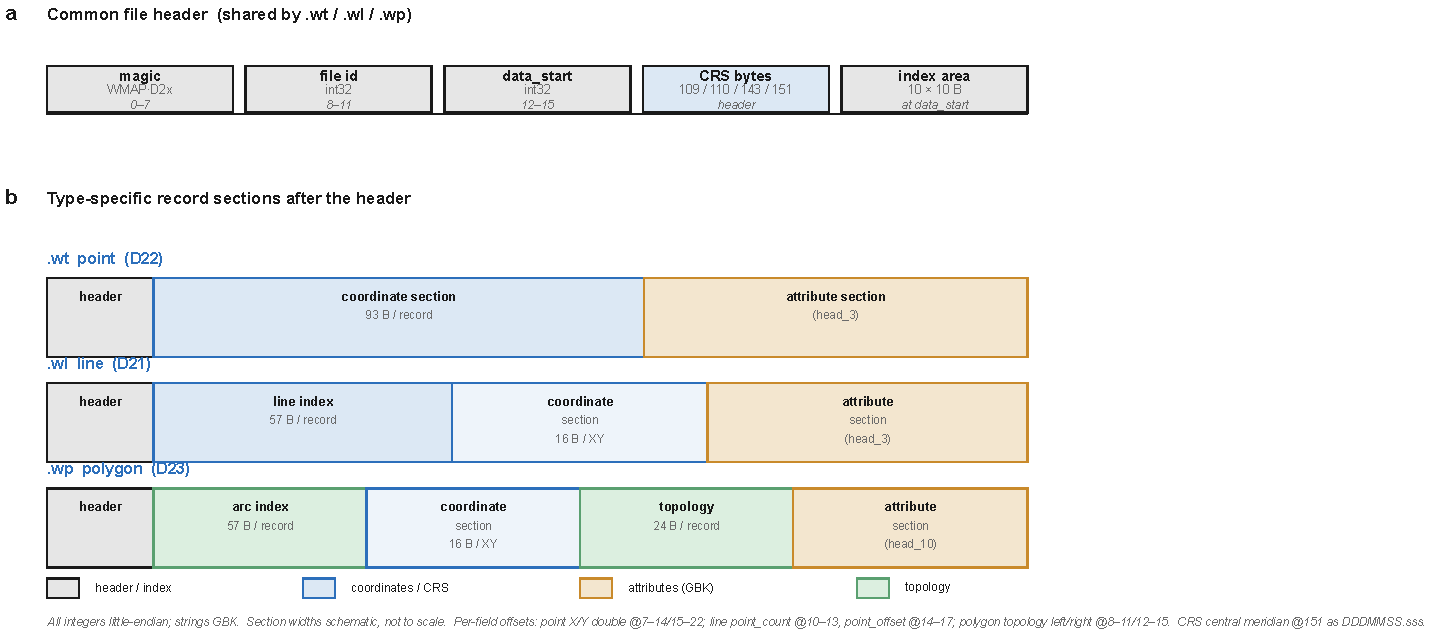
\includegraphics[width=\textwidth]{figure1_format_layout}
\caption{Byte-level layout of the MapGIS 6.x/67 vector formats. \textbf{(a)} Common file header: 8-byte magic (\texttt{WMAP`D22}/\texttt{WMAP`D21}/\texttt{WMAP`D23} for point/line/polygon), file identifier, \texttt{data\_start} offset, the coordinate-reference-system bytes (projection@109, ellipsoid@110, scale@143, central meridian@151 in \texttt{DDDMMSS.sss}), and the 10-entry index area located at \texttt{data\_start}. \textbf{(b)} Type-specific record sections: \texttt{.wt} point coordinate records (93~B; X/Y doubles at offsets 7--14/15--22), \texttt{.wl} line index (57~B) plus 16-B XY coordinate pairs, and \texttt{.wp} arc index (57~B), coordinate section, and 24-B topology records (left/right polygon identifiers at 8--11/12--15). Strips are schematic and not to scale; each block reports its record size. All integers are little-endian; strings are GBK.}
\label{fig:layout}
\end{figure}

\section{Design and Implementation}

\subsection{Architecture}
mapgis2shp is organised around a bidirectional vector-conversion core and two graphic-library parsers. The validated reader path remains a thin pipeline: binary I/O $\rightarrow$ record model $\rightarrow$ Shapely geometries $\rightarrow$ GeoPandas \texttt{GeoDataFrame}. A \texttt{Reader} parses the file in full on construction and exposes \texttt{.geodataframe}, \texttt{.fields}, \texttt{.crs}, \texttt{.bbox}, and \texttt{.to\_file()}. A \texttt{Writer} and its \texttt{write()} convenience function provide the reverse path from a \texttt{GeoDataFrame} to \texttt{.wt}, \texttt{.wl}, or \texttt{.wp}. The command-line interface selects the conversion direction from the input extension, while \texttt{pymapgis lib} inspects \texttt{Subgraph.lib} and \texttt{LINESTY.lib}. The package targets Python~$\geq$~3.9 and depends on geopandas, numpy, pandas, pyogrio, pyproj, and shapely. Figure~\ref{fig:arch} illustrates the validated reader core; the write and graphic-library paths are described in the following subsections.

\subsection{Vectorised binary parsing}
Binary records are decoded using NumPy structured dtypes rather than per-field \texttt{struct.unpack} calls. The point, arc-index, and topology tables are each materialised in a single \texttt{np.frombuffer} call, and coordinate arrays are reshaped to $(n,2)$ and scaled vectorially. Attribute-table field descriptors are unpacked in bulk through a precompiled \texttt{struct.Struct} that mirrors the 39-byte descriptor layout.

\subsection{Coordinate-reference inference}
From the projection index (byte~109) and the ellipsoid index (byte~110), mapgis2shp constructs a PROJ string. Longitude/latitude files (projection~0) yield a geographic CRS; Transverse Mercator~(5), Albers~(2), and Lambert~(3) yield projected CRSes, with the central meridian decoded arithmetically from the \texttt{DDDMMSS.sss} double (thereby preserving fractional seconds and handling western longitudes correctly). Supported ellipsoid codes include Krassovsky-based Beijing~1954, Xi'an~1980, WGS84, and WGS72. When the projection or ellipsoid code is unrecognised, or the scale is zero, the reader returns no CRS (\texttt{None}) rather than guessing, so that downstream code can detect the gap.

\subsection{Polygon topology reconstruction}
Polygon geometries are rebuilt from the arc--node topology. Arcs whose left or right polygon identifier equals the target identifier are oriented consistently, chained into closed rings by endpoint matching, and classified into shells and holes by containment. Ring assembly uses a spatial hash on arc endpoints (cell size $10^{-5}$ map units) combined with a two-sided greedy walk and a closure-competition rule, which reduces the merge from $O(n^{3})$ (a fresh all-pairs distance matrix at every iteration) to $O(n)$ in the common case while preserving the semantics of the original nearest-pair heuristic. Rings that fail to close cleanly---a known artefact of topological gaps in the source data---are passed through \texttt{shapely.make\_valid} to repair their geometry; degenerate rings with fewer than four coordinates are skipped.

\begin{figure}[h]
\centering
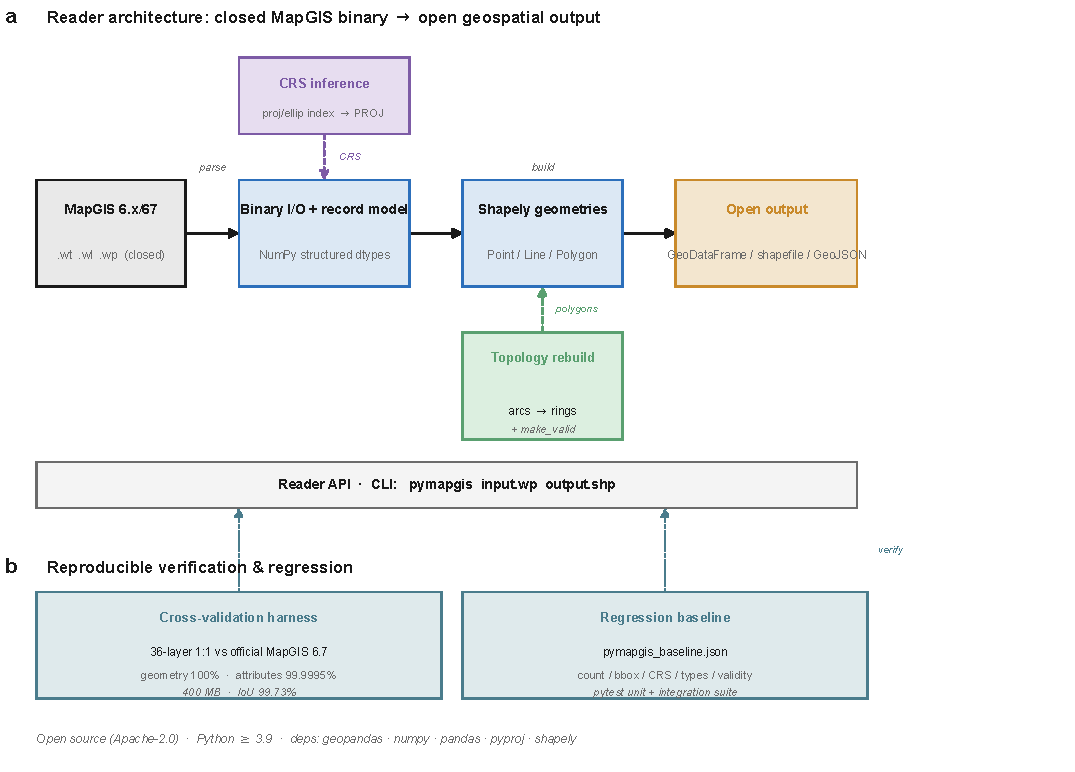
\includegraphics[width=\textwidth]{figure2_architecture}
\caption{Core reader architecture and verification resources. \textbf{(a)} Validated reader path: MapGIS \texttt{.wt}/\texttt{.wl}/\texttt{.wp} binary input $\rightarrow$ binary I/O and record model $\rightarrow$ Shapely geometries $\rightarrow$ open outputs, with CRS-inference and polygon-topology side paths. The CLI bar shows a reader-direction example. \textbf{(b)} Native-validation and regression resources. The displayed 99.9995\% attribute value is the unweighted mean of the 36 per-layer equivalence rates; the pooled cell-level rate is 99.9979\%. Version 2.4.0 additions not drawn here are the Writer, bidirectional CLI dispatch, expanded graphic-parameter decoding, graphic-library parsers, and the pyogrio dependency used for GIS-file input.}
\label{fig:arch}
\end{figure}

\subsection{Native-format writing and regression scope}
The \texttt{Writer} serialises geometries, typed attributes, supported CRS definitions, and available graphic-parameter columns into native \texttt{.wt}, \texttt{.wl}, or \texttt{.wp} sections. For polygons, it regenerates arc--node topology and stores a shared boundary as a single arc with left/right polygon identifiers. The repository's \texttt{verify\_pymapgis.py -{}-roundtrip} procedure checks Reader--Writer--Reader consistency using feature counts, bounding boxes, and polygon areas, while the test suite covers attribute types, graphic-parameter round trips, topology regeneration, CLI dispatch, and library parsing. These are internal regression checks, not independent validation by the proprietary MapGIS application.

\subsection{Graphic parameters and graphic-library structures}
With \texttt{read\_graphic\_params=True}, the reader exposes stored drawing parameters in addition to geometry and attributes. Point parameters distinguish text and symbol points and include symbol number, glyph dimensions, rotation, colour, layer, and kind-dependent font or pen-width fields. Line parameters include primary and auxiliary style numbers, line and auxiliary colours, width, pattern coefficients, layer, and transparent-output flags. Polygon parameters expose fill colour, pattern number, and the full unsigned 16-bit pattern colour. The 2.4.0 field layouts were aligned with MapGIS plain-text exports and pinned by byte-level regression tests.

\texttt{SubgraphLib} parses indexed and supported chained-tail symbol records into subpaths and fitted circle primitives; \texttt{LinestyLib} parses sublines, element templates, dot/dash rhythms, and pen parameters. These APIs expose structural drawing information for downstream use. They do not infer geological semantics, and they do not by themselves establish vendor-identical rendering. Symbol, style, colour, and pattern numbers remain library-local and must be resolved against the library version that produced the data.

\section{Validation}
This section first quantifies how closely the core reader output matches the reference implementation (official MapGIS) on real production data and then measures reader runtime and memory on the 36-layer corpus. The native-export experiments predate the 2.4.0 write and graphic-library extensions and therefore support reader fidelity only; they do not establish native acceptance of written files or vendor-identical rendering.

\subsection{Dataset}
The validation set comprises \textbf{36 MapGIS vector layers} drawn from a 1:50{,}000 geological-survey sheet in the Kurgan region (J43C001002, Xinjiang, China): 5 point layers, 18 line layers, and 13 polygon layers, totalling \textbf{16{,}874 features} (Table~\ref{tab:dataset}). The layers span geological boundaries, faults, attitudes, hydrology, and Quaternary geology, and range from small (2-feature) to large (6{,}981-feature) files.

\begin{table}[h]
\centering
\caption{Validation dataset (36 layers; abbreviated).}
\label{tab:dataset}
\begin{tabular}{llr}
\toprule
Layer & Type & Features \\
\midrule
LDLYAAI002 & point & 242 \\
LDLYAAE001 & line & 1{,}143 \\
LDZOFBB001 & polygon & 608 \\
LFZYBCT001 & point & 6{,}981 \\
LDZOFBA002 & line & 2{,}222 \\
\multicolumn{2}{l}{\emph{(31 further layers)}} & --- \\
\midrule
\textbf{Total} & \textbf{5 pt / 18 ln / 13 poly} & \textbf{16{,}874} \\
\bottomrule
\end{tabular}
\end{table}

\subsection{Protocol}
Each layer was processed in two ways: (i) read with mapgis2shp to produce a \texttt{GeoDataFrame}, and (ii) exported to ESRI shapefile using the official MapGIS 6.7 software (Zondy Cyber) under default export settings. The two outputs were then aligned by the unique \texttt{ID} attribute and compared along four axes:
\begin{itemize}
  \item \textbf{Count}: feature counts.
  \item \textbf{Schema}: attribute column-name sets.
  \item \textbf{Geometry}: point distance, line Hausdorff distance, and polygon intersection-over-union (IoU). Point and line pairs are deemed coincident at a tolerance of $10^{-7}$~degrees; polygon pairs require $\mathrm{IoU}\geq 1-10^{-6}$.
  \item \textbf{Attributes}: per-field semantic equivalence, using a classifier that distinguishes exact matches from cases in which the native export is lossy (floating-point truncation, numeric formatting, or whitespace stripping) and from genuine mismatches.
\end{itemize}
The full protocol is implemented in \texttt{cross\_validate\_native.py}, preserved in the historical repository record linked under Data Availability. Repeating the reported comparison requires access to the survey layers and the official MapGIS software; the current repository also provides synthetic fixtures for tests that do not require the restricted source data.

\subsection{Results}
Across all 36 layers and 16{,}874 features:
\begin{itemize}
  \item \textbf{Feature counts} are identical for 36/36 layers (16{,}874~=~16{,}874).
  \item \textbf{Schemas} are identical for 36/36 layers (every attribute column name matches).
  \item \textbf{Geometry} matches for 100\% of aligned features. Point distances and line Hausdorff distances are zero within $10^{-7}$ degrees, and the reported polygon IoU is 1.0 for every aligned polygon pair.
  \item \textbf{Attributes}: treating exact matches and classified native-export losses as equivalent gives a 99.9995\% unweighted mean of the 36 per-layer rates. Pooling instead across all compared cells gives 95{,}004 equivalent cells out of 95{,}006 (99.9979\%). The two residual mismatches are floating-point values smaller than $10^{-6}$ (for example, $6.69\times10^{-7}$ in mapgis2shp versus $1\times10^{-6}$ in the native export), consistent with coarse native rounding rather than a reader-originated semantic change.
  \item \textbf{CRS}: mapgis2shp reconstructs and attaches a Krassovsky-based CRS with the expected \texttt{towgs84} parameters; the examined native shapefile exports contain \textbf{no \texttt{.prj} file}, so their CRS metadata are absent.
\end{itemize}

Table~\ref{tab:results} summarises these results.

\begin{table}[h]
\centering
\caption{Cross-validation results (summary across 36 layers).}
\label{tab:results}
\begin{tabular}{ll}
\toprule
Metric & Result \\
\midrule
Layers compared & 36 \\
Features (mapgis2shp / native) & 16{,}874 / 16{,}874 \\
Count match & 36 / 36 \\
Schema match & 36 / 36 \\
Geometric coincidence & 100\% (36 / 36 layers) \\
Attribute equivalence (layer mean / pooled) & 99.9995\% / 99.9979\% \\
Residual mismatches & 2 / 95{,}006 cells \\
CRS attached & mapgis2shp yes; native no \\
\bottomrule
\end{tabular}
\end{table}

\subsection{Source information lost in the examined native export}
In 10{,}245 of the 95{,}006 compared cells (10.8\%), mapgis2shp preserves source information that the native shapefile export discards (Table~\ref{tab:lossy}):
\begin{enumerate}
  \item \textbf{Floating-point truncation}: the native export rounds floats to 2--6 significant figures (for example, $0.6218423 \rightarrow 0.62$ and $4.88\times10^{-6} \rightarrow 5\times10^{-6}$), whereas mapgis2shp preserves full double precision.
  \item \textbf{Numeric formatting}: values stored as floating-point are exported by MapGIS as integer strings in some fields (for example, \texttt{72.0} versus \texttt{72}); mapgis2shp preserves the stored type.
  \item \textbf{String padding}: the native export strips leading and trailing whitespace that the binary field actually stores (for example, \texttt{'113000\quad'} $\rightarrow$ \texttt{'113000'}), whereas mapgis2shp preserves the raw bytes.
\end{enumerate}
For these comparisons, the reader therefore retained source information that the examined native export discarded. This conclusion concerns the tested export path and does not imply that every MapGIS export option is lossy.

\begin{table}[h]
\centering
\caption{Categories of native-export lossy artefacts (10{,}245 classified cells in total).}
\label{tab:lossy}
\begin{tabular}{ll}
\toprule
Category & Example (mapgis2shp $\rightarrow$ native) \\
\midrule
Float truncation & $0.6218423 \rightarrow 0.62$ \\
Sci-notation rounding & $4.88\times10^{-6} \rightarrow 5\times10^{-6}$ \\
Numeric formatting & \texttt{72.0} $\rightarrow$ \texttt{72} \\
Whitespace stripping & \texttt{'113000\quad'} $\rightarrow$ \texttt{'113000'} \\
\bottomrule
\end{tabular}
\end{table}

\subsection{Large-file coverage validation}
\label{sec:largescale}
To stress the reader beyond the 36 survey layers, a single 400~MB MapGIS polygon file (78{,}873 features) was compared against an official MapGIS export of the same source. Because the official export had been post-processed (adjacent polygons dissolved and re-coloured), a 1:1 feature-wise comparison is impossible; coverage equivalence was therefore assessed through geometric unions, with areas computed on the Krassovsky ellipsoid using \texttt{pyproj.Geod} to avoid a costly reprojection of the full geometry set.

The results were as follows:
\begin{itemize}
  \item \textbf{Bounding box}: exact match (difference~$=$~0).
  \item \textbf{CRS}: correctly inferred as Beijing-1954 / Krassovsky (longlat)---the official export had lost its \texttt{.prj} file.
  \item \textbf{Attribute fields}: the 16 native fields are identical; the official export carries two additional fields (\texttt{strat\_code} and \texttt{ColorCode}) that are artefacts of its dissolve-and-recolour post-processing.
  \item \textbf{Invalid geometries}: mapgis2shp produced 0; the official export produced 3.
  \item \textbf{Coverage equivalence}: the union symmetric difference is 5{,}649.94~km$^{2}$ against $2.11\times10^{6}$~km$^{2}$ of coverage, giving a \textbf{coverage IoU of 99.73\%}.
\end{itemize}
The summed polygon areas differ by 1.66\% (mapgis2shp being larger), but this is an overlap artefact of the greedy arc-merge reconstruction at shared boundaries (sliver bridging across topological gaps), not a coverage error: once overlaps are removed by the union, the real coverage difference is only 0.27\%. Table~\ref{tab:large} summarises the large-file comparison.

\begin{table}[h]
\centering
\caption{Large-file (400~MB, 78{,}873 features) validation against the official MapGIS export.}
\label{tab:large}
\small
\begin{tabular}{lll}
\toprule
Metric & mapgis2shp / Official & Agreement \\
\midrule
File size & 400~MB / 327~MB shp & --- \\
Features & 78{,}873 / 67{,}039 (dissolved) & counts differ (post-processing) \\
Bounding box & $[73.486, 32.0, 111.000, 48.0]$ & exact (diff~$=$~0) \\
CRS & Krassovsky / Beijing-54 (inferred) & correct \\
Native attribute fields & 16 / 16 (+2 post-process) & 16 identical \\
Invalid geometries & 0 / 3 & 0 versus 3 \\
Union symmetric difference & --- & 5{,}649.94~km$^{2}$ (0.27\% of coverage) \\
\textbf{Coverage IoU} & --- & \textbf{99.73\%} \\
Summed-area gap & +1.66\% & overlap artefact \\
\bottomrule
\end{tabular}
\end{table}

\subsection{Reader performance and memory use}
\label{sec:performance}
We benchmarked the current 2.4.0 source on a Windows~10 workstation with a 12th-generation Intel Core i9-12950HX processor (16 physical cores, 24 logical processors), 31.7~GiB of physical memory, and CPython~3.14.6. The benchmark used default \texttt{Reader} settings: geometry repair was enabled and optional graphic-parameter decoding was disabled. For each layer, a fresh Python process performed three consecutive reads, and the full 36-layer sequential pass was repeated three times in a separate process. Reported times are medians; they exclude package import but include \texttt{Reader} construction and \texttt{GeoDataFrame} access. Memory was measured as the Windows peak working set using \texttt{psutil}, with the post-import RSS retained as a baseline. Repeated reads may benefit from operating-system file caching, so these are repeated-read rather than cold-disk measurements.

The full corpus occupied 9.17~MiB on disk and was read sequentially in a median of 0.8477~s (individual corpus passes: 0.8350--0.8639~s), corresponding to 19{,}907 features/s and 10.81~MiB/s. Absolute peak working set was 129.5~MiB, compared with a 107.3~MiB post-import baseline, giving an incremental peak of 22.2~MiB. Table~\ref{tab:performance} reports the corpus and the largest layer of each geometry type by feature count. The 608-feature polygon layer was both the slowest individual layer (0.3718~s) and had the largest per-layer incremental peak (21.8~MiB), consistent with polygon arc--node reconstruction being the dominant cost in this corpus. These measurements cover the 36-layer reader corpus only; they do not benchmark the \texttt{Writer}, native MapGIS software, or the 400~MB file.

\begin{table}[h]
\centering
\caption{Reader runtime and memory results (median of three reads; $\Delta$peak is the peak working-set increment above the post-import baseline).}
\label{tab:performance}
\small
\begin{tabular}{llrrrr}
\toprule
Layer & Type & Features & Input (MiB) & Time (s) & $\Delta$peak (MiB) \\
\midrule
LFZYBCT001 & point & 6{,}981 & 1.31 & 0.0683 & 8.4 \\
LFZYBCT002 & line & 2{,}331 & 0.55 & 0.0311 & 4.7 \\
LDZOFBB001 & polygon & 608 & 2.07 & 0.3718 & 21.8 \\
\midrule
\textbf{All 36 layers} & \textbf{corpus} & \textbf{16{,}874} & \textbf{9.17} & \textbf{0.8477} & \textbf{22.2} \\
\bottomrule
\end{tabular}
\end{table}

\section{Comparison with prior tools}
Table~\ref{tab:tools} compares mapgis2shp with the prior open-source MapGIS readers and the Chinese academic precedents using capabilities documented in the cited sources: licence, implementation language, byte-level specification, CRS inference, and independent validation against the reference implementation. Within this comparison set, mapgis2shp is the only entry that combines CRS inference with quantified native-export validation and an installable, regression-tested package. A ``no'' denotes a capability not reported in the cited source rather than proof that it is impossible or absent from every version.

\begin{table}[h]
\centering
\caption{Documented capabilities of the tools and publications examined.}
\label{tab:tools}
\begin{tabular}{llllccc}
\toprule
Tool & Year & Lang & Licence & Spec & CRS & Validated \\
\midrule
pymapgis (predecessor) & 2022 & Python & none & yes & no & no \\
MathsionYang & 2019 & C\# & --- & no & no & no \\
ConvertMapGIS & 2025 & Python & GPL-3.0 & yes & no & no \\
OGC.net & 2021 & C\# & none & no & no & no \\
Wang (2013) & 2013 & --- & n/a & no & no & no \\
\textbf{mapgis2shp} & 2026 & Python & Apache-2.0 & yes & \textbf{yes} & \textbf{yes} \\
\bottomrule
\end{tabular}
\end{table}

\section{Discussion}

\subsection{Limitations}
\label{sec:discussion}
The reader supports the common ellipsoid codes and projections described above; unrecognised codes yield no CRS that downstream code must handle explicitly. The later MapGIS K9/10 formats are not supported because they use different layouts. CRS inference relies on the file's index codes and embedded common definitions rather than a complete external MapGIS parameter environment, so unusual projections or datums may be under-described. Moreover, the 36-layer corpus comes from one geological-survey sheet and the large-file stress test concerns one polygon dataset; the reported error rates should not be extrapolated to every MapGIS producer, object type, or export configuration.

Polygon topology reconstruction remains heuristic. Although \texttt{make\_valid} repaired the tested outputs, topological gaps can produce repaired rather than exact source polygons. In the 400~MB test, greedy arc merging introduced a 1.66\% overlap artefact in summed polygon areas at shared boundaries, corresponding to a 0.27\% union-level coverage difference. The small-file geometric results therefore do not remove the need for coverage-level checks when an exact planar partition is required at larger scales.

The write and graphic-library paths have separate validation boundaries. Reader--Writer--Reader tests do not establish that every written file will open and display correctly in MapGIS 6.7. The writer does not emit auxiliary annotation-text sections for \texttt{.wt}, supports only the CRS families listed above, and cannot preserve long graphic-parameter column names through an intermediate shapefile because of that format's 10-character field-name limit; direct \texttt{GeoDataFrame}, GeoJSON, or GeoPackage hand-off avoids that particular constraint. Finally, graphic parameters are not self-contained: their interpretation depends on the originating symbol, style, colour, and pattern libraries. Unsupported or out-of-range symbol lookups return no geometry rather than an inferred glyph, and structural library parsing is not a claim of geological semantic interpretation or pixel-identical vendor rendering.

\subsection{Generalisability}
The validation methodology---reverse-engineering a proprietary format and then cross-validating the reader against the reference implementation on real data, with quantified geometric and attribute fidelity---transfers to other closed geoscience formats. The cross-validation script is format-agnostic in structure and could anchor similar studies wherever a reference implementation is available. This generality concerns the protocol, not the numerical error rates, which remain specific to the files and export settings tested here.

\subsection{Open-science implication}
By making MapGIS 6.x/67 data readable and writable from the open-source Python stack, mapgis2shp supports reproducible analysis, format migration, and long-term archival of Chinese geological-survey data. Access to graphic parameters and library structures additionally preserves information needed to interpret the original cartography, provided the originating libraries are available. The CRS-inference capability is of particular practical importance because the examined native exports omitted projection files; users can therefore recover metadata that would otherwise require manual reconstruction.

\subsection{Literature coverage}
Searches of Crossref, OpenAlex, arXiv, and DOAJ, together with manual searches of CNKI and Wanfang, primarily retrieved MapGIS--ArcGIS conversion studies and application notes based on the vendor SDK or the documented ASCII plain-code format. Within these search results, we found no peer-reviewed report combining an open-source MapGIS 6.x/67 binary reader with independent native-export validation. This is a bounded literature-search result rather than proof that no other implementation exists; the open-source prior art identified independently of publication status is acknowledged in Section~\ref{sec:related}.

\section{Conclusions}
mapgis2shp is an open-source Python toolkit for the closed MapGIS 6.x/67 binary vector formats. Native-export comparisons support the fidelity of its reader core: across 36 real geological-survey layers (16{,}874 features), all aligned geometries met the type-specific coincidence criteria and only two residual mismatches were found among 95{,}006 compared attribute cells; on a 400~MB polygon file (78{,}873 features), coverage IoU was 99.73\%. The comparisons also show that the examined native exports discarded floating-point precision, string padding, and CRS metadata retained by the reader. Version 2.4.0 extends this validated core with native-format writing, expanded graphic-parameter decoding, and graphic-library parsers, while the remaining polygon-overlap, native-write-acceptance, and library-dependence boundaries remain explicit. The software is distributed on PyPI under the Apache-2.0 licence, with regression resources and historical validation artifacts preserved in the repository record.

\section*{Availability and Requirements}
\begin{itemize}
  \item \textbf{Software name:} mapgis2shp (import name \texttt{pymapgis})
  \item \textbf{Version described:} 2.4.0
  \item \textbf{PyPI:} \texttt{pip install mapgis2shp}
  \item \textbf{Source code:} \url{https://github.com/leecugb/mapgis2shp}
  \item \textbf{Archived DOI:} \url{https://doi.org/10.5281/zenodo.21487339}
  \item \textbf{License:} Apache-2.0
  \item \textbf{Operating systems:} Windows, Linux, macOS
  \item \textbf{Dependencies:} Python~$\geq$~3.9; geopandas~$\geq$~0.12, numpy~$\geq$~1.21, pandas~$\geq$~1.3, pyogrio~$\geq$~0.8, pyproj~$\geq$~3.2, shapely~$\geq$~2.0
\end{itemize}

\section*{Data Availability Statement}
The 36 MapGIS validation layers and the 400~MB large-file dataset are real geological-survey data from the China Geological Survey and are not redistributed with the package. The native-validation scripts and reports used in this article are preserved in the repository history at commit \texttt{d0d464d0}. The 36-layer comparison is under \path{paper/validation/} (\path{cross_validate_native.py}, \path{cross_validation_report.csv}, and \path{cross_validation_report.md}); the large-file comparison includes \path{cross_validate.py} and \path{cross_validate_large_report.md}. The permanent entry point is the \href{https://github.com/leecugb/mapgis2shp/tree/d0d464d05166ab97978a01ce8cc5cc8480f05500}{GitHub record for this commit}.

The current 2.4.0 repository separately provides the regression driver \path{verify_pymapgis.py} (including \texttt{-{}-roundtrip}), the baseline \path{pymapgis_baseline.json}, and the \path{tests/} suite. These resources cover unit, CLI, writer, graphic-parameter, and library regressions; tests requiring unavailable real-data fixtures are skipped.

The reproducible performance benchmark \path{benchmark_performance.py} and its raw outputs \path{performance_benchmark.json} and \path{performance_benchmark.csv} accompany this manuscript. These files record the hardware and software environment, every timing sample, input sizes, feature counts, and baseline, absolute-peak, and incremental-peak memory values.

\section*{CRediT author statement}
S.L. conceived and designed the study, developed the software, carried out the validation, and wrote the main manuscript text; S.L. also prepared Figures~1 and~2. H.H. contributed to the validation and reviewed the manuscript. X.S., H.Q., X.L., Y.F. and Z.Z. contributed to data investigation and reviewed the manuscript. All authors reviewed and approved the final manuscript.

\section*{Declaration of competing interests}
The authors declare no competing interests.

\section*{Funding}
This work was supported by the Deep Earth Probe and Mineral Resources Exploration - National Science and Technology Major Project (Program No.2025ZD10069).

\begin{thebibliography}{99}
\bibitem{warmerdam2008}
Warmerdam F (2008) The Geospatial Data Abstraction Library. In: Hall GB, Leahy MG (eds) Open Source Approaches in Spatial Data Handling. Advances in Geographic Information Science. Springer, Berlin, Heidelberg, pp 87--104. \url{https://doi.org/10.1007/978-3-540-74831-1_5}

\bibitem{gdalwebsite}
GDAL/OGR contributors (2026) Vector drivers list. \url{https://gdal.org/drivers/vector/index.html}. Accessed 22 July 2026.

\bibitem{pymapgis2022}
Li S (2022) pymapgis: a Python library for reading MapGIS 6.x/67 vector files. \url{https://github.com/leecugb/pymapgis}. Accessed 22 July 2026.

\bibitem{mathsionyang2019}
MathsionYang (2019) MapGIS2ArcGIS. \url{https://github.com/MathsionYang/MapGIS2ArcGIS}. Accessed 22 July 2026.

\bibitem{convertmapgis2025}
BenChao1998 (2025) ConvertMapGIS. \url{https://github.com/BenChao1998/ConvertMapGIS}. Accessed 22 July 2026.

\bibitem{ogcnet2021}
Wong W (2021) OGC.net. \url{https://github.com/WenboWong/OGC.net}. Accessed 22 July 2026.

\bibitem{wang2013}
Wang X (2013) Data analysis and reading test on MapGIS point file. Science of Surveying and Mapping (in Chinese) 2013(1):112--115.

\bibitem{wufeng2006}
Wu L, Feng J (2006) Study on the key techniques of MapGIS and Geodatabase data format conversion. Chinese Journal of Engineering Geophysics (in Chinese).

\bibitem{chen2000}
Chen H, Wu J, Wang J (2000) Realisation of format conversion in MapGIS with MATLAB. Computing Techniques for Geophysical and Geochemical Exploration (in Chinese) 22(4):351--355.

\bibitem{shotwell2011}
Shotwell M (2011) sas7bdat: sas7bdat reverse engineering documentation. CRAN (The R Foundation). \url{https://doi.org/10.32614/cran.package.sas7bdat}

\bibitem{senanayake2022}
Senanayake AI, Chandler RJ, Daly T, Lewis E (2022) python-ags4: a Python library to read, write, and validate AGS4 geodata files. Journal of Open Source Software 7(79):4569. \url{https://doi.org/10.21105/joss.04569}

\bibitem{wright1998}
Wright D, Wood R, Sylvander B (1998) ArcGMT: a suite of tools for conversion between Arc/INFO and Generic Mapping Tools (GMT). Computers \& Geosciences 24(8):737--744. \url{https://doi.org/10.1016/s0098-3004(98)00067-3}

\bibitem{sen2005}
Sen M, Duffy T (2005) GeoSciML: development of a generic GeoScience Markup Language. Computers \& Geosciences 31(9):1095--1103. \url{https://doi.org/10.1016/j.cageo.2004.12.003}

\bibitem{vandenbos2014}
van den Bos J (2014) Lightweight runtime reverse engineering of binary file format variants. In: 2014 Software Evolution Week -- IEEE CSMR-WCRE. IEEE, pp 367--370. \url{https://doi.org/10.1109/csmr-wcre.2014.6747196}

\bibitem{ma2012}
Ma Y, Wang J, Xie S (2012) Analytical application of MapGIS for quality control in geological map spatial database constructing. Geo-information Science 13(6):758--762. \url{https://doi.org/10.3724/sp.j.1047.2011.00758}

\bibitem{han2012}
Han K, Pang J, Lu Y, Ding D, Fan B, Ju Y, Wang Z (2012) Research on sharing of geological map spatial data network under the ``OneGeology'' project: taking China 1:1M geological map data in MapGIS format as an example. Geo-information Science 13(6):742--749. \url{https://doi.org/10.3724/sp.j.1047.2011.00742}
\end{thebibliography}

\end{document}
